



\section*{Introducción}

En el análisis y diseño de circuitos electrónicos, el comportamiento no lineal de ciertos componentes es un factor determinante para el funcionamiento de dispositivos modernos. Las fuentes no lineales, tanto controladas como no controladas, representan sistemas cuya respuesta en corriente o voltaje no es proporcional a la señal de entrada. Este tipo de fuentes es fundamental para entender una gran variedad de aplicaciones electrónicas, desde amplificadores hasta circuitos de radiofrecuencia.

En particular, las características \textbf{cuadráticas} y \textbf{exponenciales} son dos formas comunes de modelar el comportamiento no lineal. La característica cuadrática suele surgir en aproximaciones polinómicas de sistemas con no linealidades suaves, mientras que la característica exponencial es intrínseca a dispositivos semiconductores como diodos y transistores en polarización directa. Comprender la diferencia entre estas características es esencial para predecir el comportamiento de los circuitos y optimizar su desempeño.

Este documento aborda las principales aplicaciones de fuentes no lineales \textbf{controladas} con comportamiento exponencial, destacando su relevancia en electrónica de potencia, procesamiento de señales, comunicaciones y sensado. Posteriormente, se comparan las características cuadráticas y exponenciales en el contexto de \textbf{fuentes no lineales no controladas}, considerando sus implicaciones prácticas y el impacto en el diseño de circuitos. Finalmente, se desarrolla un problema aplicado que permite calcular los valores de resistencia y capacitancia necesarios para lograr una respuesta de salida específica en un circuito con transistor.

El análisis propuesto integra conceptos teóricos y prácticos, apoyándose en modelos matemáticos y ecuaciones fundamentales, con el fin de reforzar la comprensión del comportamiento dinámico de sistemas electrónicos no lineales.

\section{Aplicaciones de los circuitos con fuentes no lineales controladas con característica exponencial}
Las fuentes no lineales controladas con características exponenciales, como los diodos y transistores en polarización directa, tienen aplicaciones fundamentales en diversos sistemas electrónicos. Estas fuentes permiten obtener respuestas de voltaje y corriente que no siguen una relación lineal, lo cual es útil en una variedad de contextos. Algunas de sus aplicaciones principales son:

\begin{itemize}
    \item \textbf{Rectificadores y fuentes de alimentación}: Los diodos con su característica exponencial son esenciales en la conversión de corriente alterna (CA) a corriente continua (CC), gracias a su capacidad de conducir en una sola dirección.
    
    \item \textbf{Circuitos amplificadores}: En configuraciones como el transistor bipolar en modo activo, la relación exponencial entre la corriente base y la corriente colector permite la amplificación de señales pequeñas.
    
    \item \textbf{Osciladores electrónicos}: Utilizan dispositivos con características exponenciales para generar señales de oscilación de frecuencia estable, esenciales en comunicaciones y sistemas de reloj.
    
    \item \textbf{Modulación y demodulación de señales}: En telecomunicaciones, los circuitos que realizan modulación AM o FM emplean componentes no lineales para transformar señales de información.
    
    \item \textbf{Etapas de mezcla en radiofrecuencia}: Los mezcladores aprovechan la no linealidad para combinar o extraer frecuencias en sistemas de transmisión y recepción de señales.
    
    \item \textbf{Sensado y medición}: Algunos sensores electrónicos utilizan elementos con respuesta exponencial para obtener una mayor sensibilidad o rango dinámico en la medición de variables físicas.
\end{itemize}

Estas aplicaciones demuestran que el comportamiento exponencial en dispositivos no lineales no solo es una característica fundamental de su funcionamiento, sino también una herramienta valiosa para el diseño de sistemas electrónicos complejos \cite{sedra_smith}.



\section{Diferencia entre una característica cuadrática y una característica exponencial en fuentes no lineales no controladas}

\subsection{Característica Cuadrática}

Una característica cuadrática describe una relación no lineal del tipo:

\begin{equation}
    y = a x^2 + b x + c
\end{equation}

Este tipo de comportamiento es típico en sistemas cuya salida depende del cuadrado de la entrada. Es una aproximación común en modelos polinomiales de segundo orden como el modelo Volterra cuadrático, o modelos autorregresivos cuadráticos (ARQ) \cite{volterra_model}. 

En electrónica, algunos dispositivos presentan una relación del tipo:

\begin{equation}
    i = A v^2
\end{equation}

donde la corriente crece con el cuadrado del voltaje aplicado \cite{sedra_smith}.

\textbf{Implicaciones prácticas}:

\begin{itemize}
    \item Generación de armónicos pares.
    \item Permite cierta linealización local.
    \item A medida que la entrada crece, la distorsión también aumenta.
\end{itemize}

\subsection{Característica Exponencial}

Una característica exponencial describe una relación del tipo:

\begin{equation}
    y = A e^{k x}
\end{equation}

Este comportamiento es característico en dispositivos semiconductores como los diodos y transistores, donde se cumple:

\begin{equation}
    I = I_0 \left( e^{\frac{V}{V_T}} - 1 \right)
\end{equation}

\cite{sedra_smith, transistor_physics}.

\textbf{Consecuencias}:

\begin{itemize}
    \item Alta sensibilidad a pequeñas variaciones de entrada.
    \item Generación de múltiples armónicos de alto orden.
    \item Difícil de linealizar excepto en regiones muy reducidas.
\end{itemize}

\subsection{Comparación Cuadrática vs Exponencial}

\begin{table}[h]
\centering
\begin{tabular}{|l|l|l|}
\hline
\textbf{Aspecto} & \textbf{Cuadrática} & \textbf{Exponencial} \\
\hline
Relación entrada-salida & $y \propto x^2$ & $y \propto e^{kx}$ \\
Nivel de no linealidad & Moderado & Alto \\
Armónicos generados & Principalmente pares & Altos armónicos múltiples \\
Linealización & Posible localmente & Limitada a baja pendiente \\
Ejemplo típico & Modelo Volterra & Diodo, transistor \\
\hline
\end{tabular}
\caption{Comparación entre características cuadráticas y exponenciales}
\end{table}

\subsection{Aplicación en fuentes no lineales no controladas}

Las fuentes \textbf{no lineales no controladas} son aquellas que no emplean retroalimentación ni técnicas de corrección. En este contexto:

\begin{itemize}
    \item Una fuente con \textbf{característica cuadrática} mostrará una salida moderadamente distorsionada, predecible dentro de un rango.
    \item Una fuente con \textbf{característica exponencial} puede exhibir inestabilidad, saturación y una respuesta extremadamente sensible, lo que dificulta su uso sin control activo.
\end{itemize}


\section{Cálculo de $R$ y $C$ a partir de la Figura \ref{fi1}, dado que $v_i(t) = \cos(10t)$ V, para obtener $v_o(t) = -10 + 13 \cos(10^7 t)$ V}

\begin{figure}[h]
    \centering
    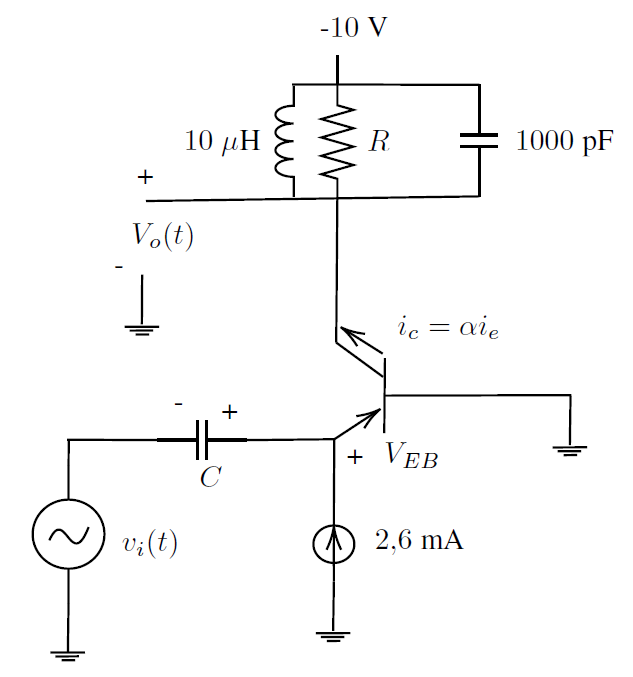
\includegraphics[width=0.75\linewidth]{circuito .png}
    \caption{Circuito de laboratorio.}
    \label{fi1}
\end{figure}
\section*{Datos del problema}
\begin{itemize}
    \item Voltaje de entrada: \( v_i(t) = \cos(10^7 t) \, \text{V} \)
    \item Voltaje de salida: \( v_o(t) = -10 + 13 \cos(10^7 t) \, \text{V} \)
    \item Inductor: \( L = 10 \, \mu\text{H} \)
    \item Capacitor: \( C_1 = 1000 \, \text{pF} \)
    \item Corriente de emisor: \( I_E = 2.6 \, \text{mA} \)
    \item Relación de corriente: \( i_c = \alpha i_e \)
\end{itemize}


\subsection{Solución}

El circuito consta de un transistor BC547 con una configuración que incluye un inductor (\( L \)), una resistencia (\( R \)), y capacitores (\( C \) y \( C_1 \)). El voltaje de entrada \( v_i(t) \) se aplica a través del capacitor \( C \), y el voltaje de salida \( v_o(t) \) se mide en el colector.

El voltaje de salida tiene un componente DC (\( -10 \, \text{V} \)) y un componente AC (\( 13 \cos(10^7 t) \, \text{V} \)).

\subsubsection*{Componente DC:}
\begin{itemize}
    \item El voltaje DC en el colector es \( -10 \, \text{V} \).
    \item La corriente de colector DC (\( I_C \)) se calcula usando \( I_C = \alpha I_E \). Para un transistor típico, \( \alpha \approx 0.98 \):
    \[
    I_C = 0.98 \times 2.6 \, \text{mA} = 2.548 \, \text{mA}
    \]
    \item La resistencia \( R \) se calcula usando la ley de Ohm:
    \[
    R = \frac{V_{CC} - V_{C}}{I_C} = \frac{0 - (-10)}{2.548 \times 10^{-3}} \approx 3924 \, \Omega
    \]
    Se recomienda usar un potenciómetro de \( 5 \, \text{k}\Omega \) para ajustar este valor.
\end{itemize}

\subsubsection*{Componente AC:}
\begin{itemize}
    \item La ganancia de voltaje \( A_v \) es:
    \[
    A_v = \frac{v_o(\text{AC})}{v_i(\text{AC})} = \frac{13}{1} = 13
    \]
    \item La impedancia del inductor \( L \) a \( \omega = 10^7 \, \text{rad/s} \):
    \[
    Z_L = j\omega L = j \times 10^7 \times 10 \times 10^{-6} = j100 \, \Omega
    \]
    \item La impedancia del capacitor \( C_1 \):
    \[
    Z_{C_1} = \frac{1}{j\omega C_1} = \frac{1}{j \times 10^7 \times 1000 \times 10^{-12}} = -j100 \, \Omega
    \]
    \item La impedancia total en paralelo \( Z_{L} \parallel Z_{C_1} \):
    \[
    Z_{\text{total}} = \frac{Z_L \cdot Z_{C_1}}{Z_L + Z_{C_1}} = \frac{(j100)(-j100)}{j100 - j100} = \infty
    \]
    Esto indica que \( L \) y \( C_1 \) forman un circuito resonante paralelo con impedancia infinita a esta frecuencia.
    \item La ganancia \( A_v \) está determinada por:
    \[
    A_v = \left| \frac{R}{\frac{1}{j\omega C}} \right| = \omega R C
    \]
    Sustituyendo \( A_v = 13 \) y \( \omega = 10^7 \):
    \[
    13 = 10^7 \times 3924 \times C \implies C \approx 3.31 \times 10^{-10} \, \text{F} = 331 \, \text{pF}
    \]
    Se recomienda probar con capacitores cercanos a \( 330 \, \text{pF} \).
\end{itemize}

\section*{Resultados finales}
\[
\boxed{R \approx 3.9 \, \text{k}\Omega \quad \text{(usar potenciómetro de 5 k}\Omega\text{)}}
\]
\[
\boxed{C \approx 330 \, \text{pF}}
\]
